\section{Introduction}
\label{sec:intro}

\begin{figure*}[t]
  \centering
  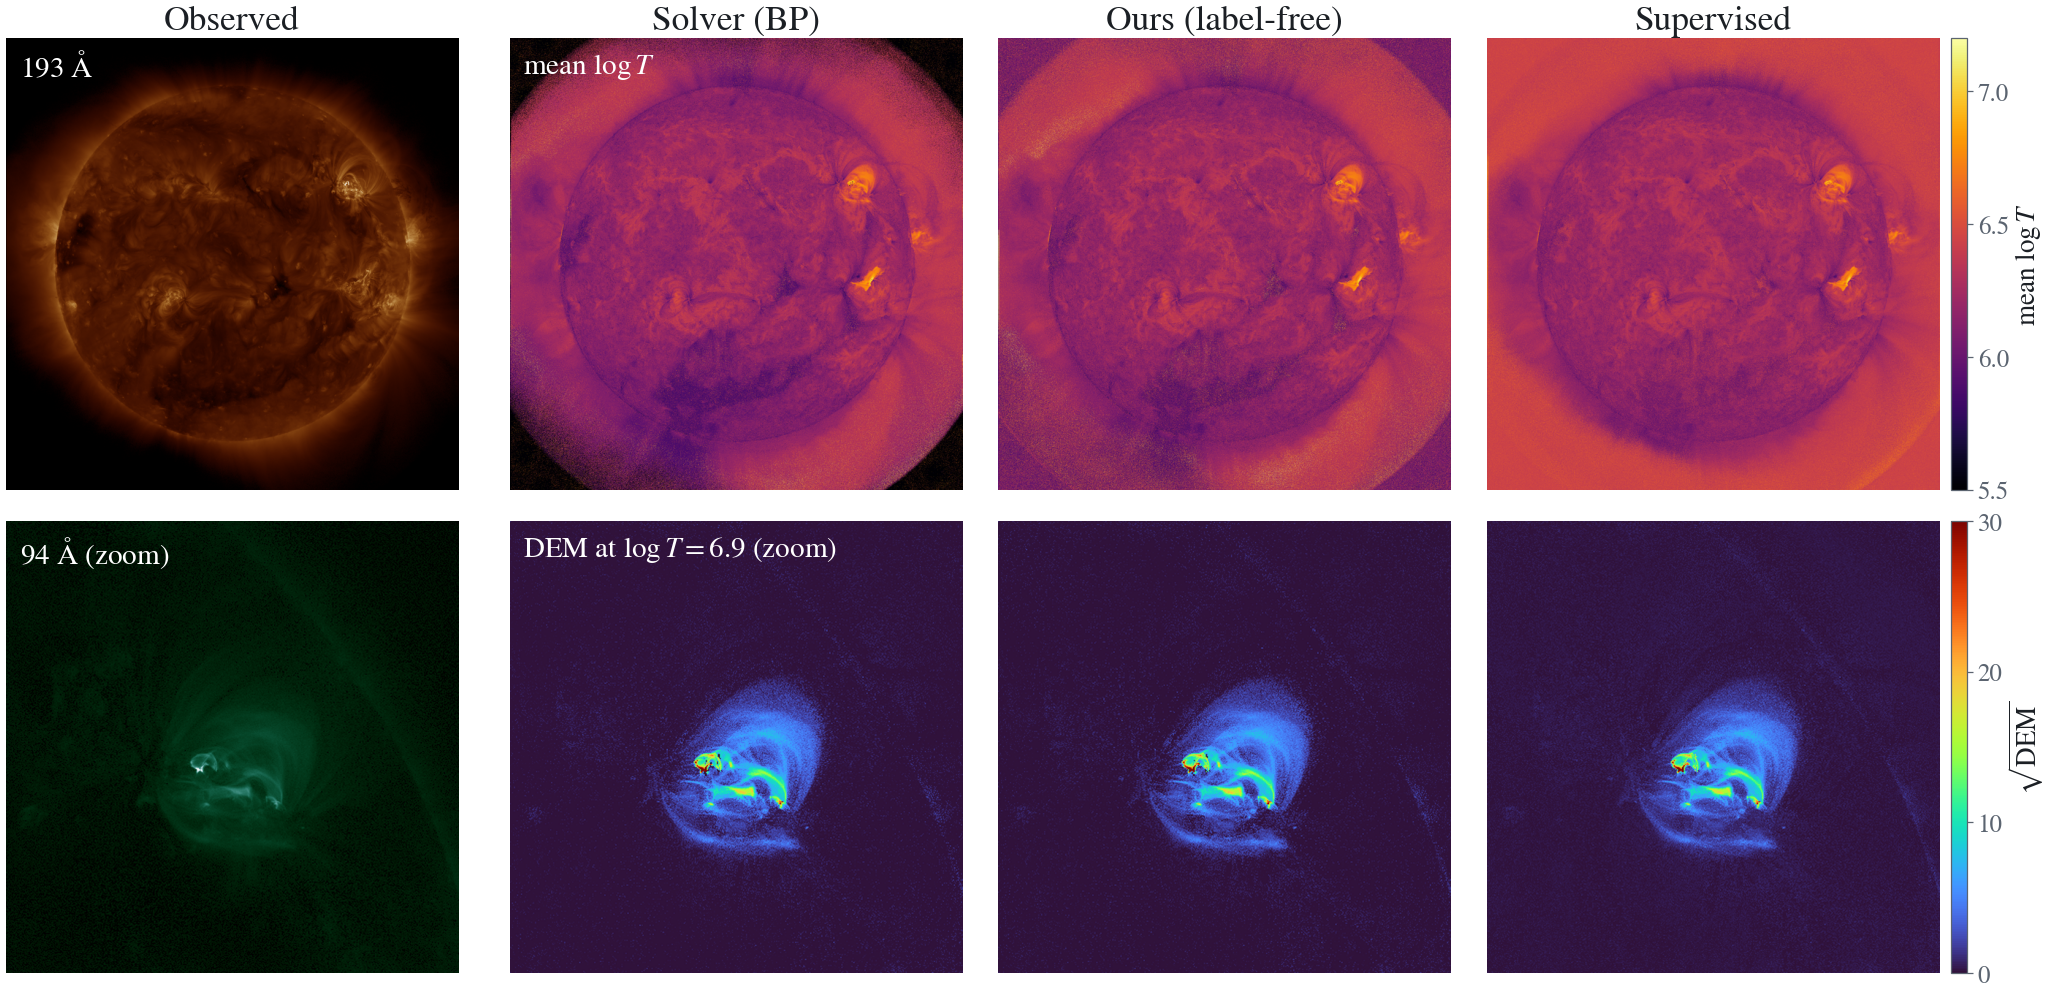
\includegraphics[width=\linewidth]{fig_disk.png}
  \caption{One held-out image from 30 September 2015. Top: the observed 193\Ang{} channel and the mean \logT{} of the DEM from the BP solver, our label-free model and the supervised baseline. Bottom: a zoom on an active region in the observed 94\Ang{} channel, and the DEM in the bin at $\logT=6.9$ (8\,MK). Our model never saw a solver DEM in training. We blank pixels flagged by the self-check of \cref{sec:capacity} in our maps.}
  \label{fig:disk}
\end{figure*}

The corona radiates in the extreme ultraviolet (EUV), and the brightness of each spectral channel depends on how much plasma lies along the line of sight at the temperatures that channel responds to. The differential emission measure (DEM) inverts this relation. For each line of sight it gives the amount of plasma per temperature bin, separating the corona near 1\,MK from flare plasma near 8\,MK, and it is a standard diagnostic of coronal thermal structure. The Atmospheric Imaging Assembly (AIA)~\cite{lemen2012aia} on the Solar Dynamics Observatory~\cite{pesnell2012sdo} images the full Sun at $4096\times4096$ pixels every 12 seconds in seven EUV channels, six of which serve DEM inversion, so in principle one can estimate a DEM for every pixel of every image.

The inversion is both slow and ill-posed. Six intensities cannot determine a DEM on 18 temperature bins, a difficulty known for fifty years~\cite{craig1976limitations}, so every solver adds a regularizer and its answer depends on that choice. We work with two. Basis Pursuit (BP)~\cite{cheung2015dem} finds the smallest total weight on a fixed basis that reproduces every channel within a noise band, which is a linear program (LP). Elastic Net~\cite{athiray2024enet} fits the same basis by regularized least squares. Both solve one problem per pixel. On our $2048\times2048$ grid a BP image is 4.2 million LPs, and one job, including deconvolution and retries, took 9.5 minutes on 16 cores. Inverting 1,223 images with both solvers took 2,446 cluster jobs and produced 1.74\,TB.

Neural emulators move this cost into training. DeepEM~\cite{wright2019deepem} regressed BP's output from AIA intensities, and DEMNet~\cite{perezdiaz2026demnet} extends the idea with Fourier-feature inputs, an uncertainty head and a final stage of forward-model finetuning. Inference becomes one forward pass, but such a model stays bound to its labels. It needs solver output for every training image, a change of solver settings invalidates that output (we discarded 886\,GB of our own Elastic Net labels when the reference regularization weight changed), and the network learns whatever the solver did, including fits to instrument artifacts.

We remove the labels. We train a per-pixel network to minimize the solver's own objective, on about 30 million pixels per epoch. This is amortized optimization~\cite{amos2023tutorial}: instead of searching for each pixel's solution, we learn a function that maps an observation to it. The objective needs only the observations, their noise and the instrument response, so no solver DEM enters training. Solver output appears only through a validity flag, a screen used to choose one loss weight, and the final evaluation, which also informed five model choices. \Cref{fig:disk} shows the result on an image the model never saw.

Removing the labels moves the difficulty into the loss. Elastic Net is already smooth, but BP has a hard constraint, which we replace by a squared penalty with weight $\mu$. Our first BP models used $\mu=1$ and looked excellent on the typical pixel, yet at flare cores they held only 40\% of the solver's emission. Oversampling those pixels, longer training and a 10M-parameter network did not help. The loss was at fault: at $\mu=1$ it charges more to keep the hot plasma than to leave it out (\cref{fig:curves}).

We make three contributions.
\begin{itemize}
\item \textbf{Label-free inversion at full-disk scale.} A per-pixel MLP trained only on the solver's objective. On 153 held-out images, against a supervised baseline scored on the same pixels, it leads on five of six headline measures on Elastic Net and ties the sixth, and it leads on four of six on BP with a median pixel error 3.6 times lower (\cref{sec:comparison}). To our knowledge no earlier DEM network trains without solver labels.
\item \textbf{A calibration of the penalty weight.} Building on a classical result for penalized LPs~\cite{mangasarian2004newton}, we give the distance each channel settles outside its band and the threshold above which that distance is exact, both computable without training a network (\cref{sec:law,sec:verify}). Comparing a network with the per-pixel minimizer of its loss, an amortization gap~\cite{cremer2018inference}, then separates loss failures from training failures. This located our flare-core failure in the loss (\cref{sec:gap,sec:flare}).
\item \textbf{An account of capacity blow-ups.} Wider models failed by orders of magnitude on a few pixels out of 705 million. Most of those pixels were inputs our own training mask had removed, and masking single channels instead of dropping whole pixels removes most of the score blow-ups, though not the most extreme reconstructions. One flare pixel dominated the worst score and is not explained this way (\cref{sec:capacity}).
\end{itemize}
